\chapter{Building an AI-First Organization}

\begin{center}
    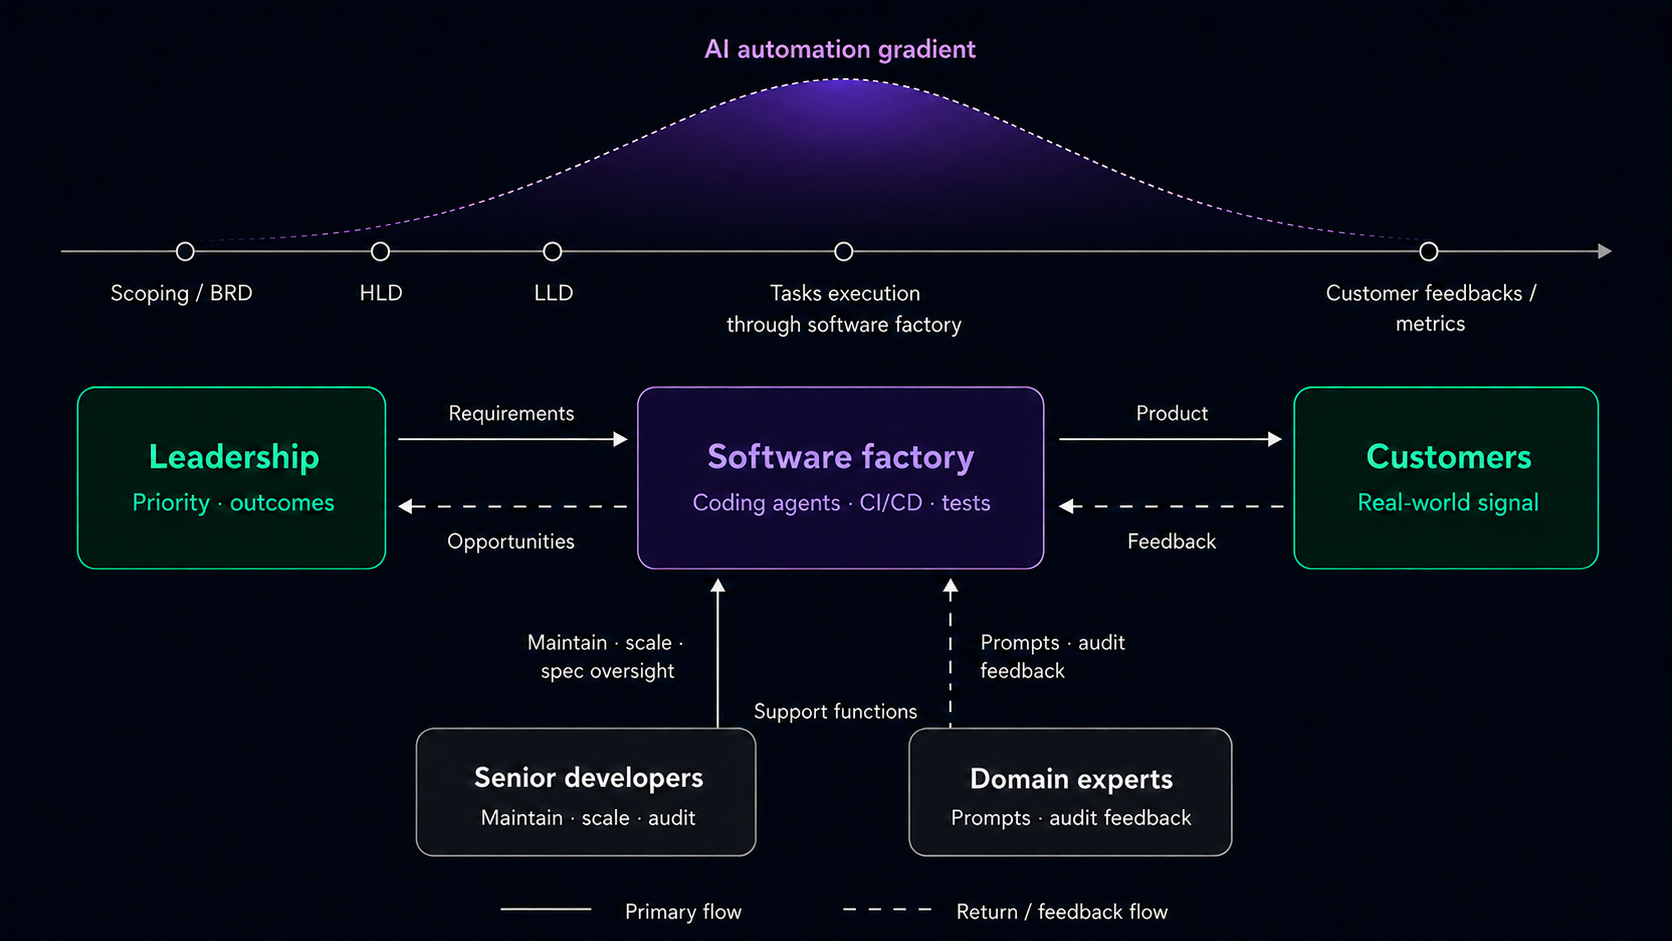
\includegraphics[width=0.9\textwidth]{figures/ai_first_company_organization.png}

    {\small The automation gradient}
\end{center}

In modern enterprise product development, the operating model can be represented as one continuous loop:

\begin{center}
\textit{business problem identification}
$\rightarrow$
\textit{BRD}
$\rightarrow$
\textit{HLD}
$\rightarrow$
\textit{LLD}
$\rightarrow$
\textit{tasks}
$\rightarrow$
\textit{implementation}
$\rightarrow$
\textit{execution}
$\rightarrow$
\textit{feedback}
$\rightarrow$
\textit{new tasks or updated business problem/design}.
\end{center}

In an AI-first company, automation follows an \textit{AI gradient}. The center of the loop is the most automatable because it is more technical, structured, and repeatable. The edges of the loop remain the most human-intensive because they require judgment, ambiguity resolution, and accountability.

At the beginning of the loop, humans identify the business problem, set the priority, and define the expected outcome. This is where human expertise is hardest to replace: identifying the right problem before it is fully specified, inferring what is unspoken, anticipating risks before they appear, and recognizing opportunities that are not yet obvious from the data.

As work moves toward the center of the loop, AI can take on more of the implementation work. It can help convert a business requirement document into a high-level design, a high-level design into a low-level design, and a low-level design into executable tasks. Coding agents can then implement the required software changes through the software factory. In this context, the software factory is the set of skills, tools, tests, and CI/CD mechanisms that allow coding agents to generate software compliant with company requirements.

The system leverages feedback signals such as SME audits through sampling, customer feedback, and actuals data. These signals are converted into metrics that compare current performance against the ideal state. Based on the gap, the AI agent decides the next action. If the gap is small or localized, it creates a new task. If the gap suggests a deeper issue in the business logic or system design, it brings the problem back to the leadership and proposes updates to the business problem, BRD, HLD, or LLD.

\section{Minimum Architecture}

The minimum architecture requires three components.

The first component is the \textit{software factory}. This is the engine that converts structured tasks into production-grade software. It uses coding agents, tests, CI/CD, and deployment gates to generate changes that are compliant with company requirements.

The second component is a small set of \textit{MCP interfaces} that allow humans and AI to communicate through the systems where work already happens. In a first version, these interfaces can connect to Asana, Outlook/Mail, and Slack. Asana acts as the execution surface, while Outlook and Slack act as communication surfaces.

The third component is the \textit{knowledge base}. This stores the key documents and context required by the AI system, including BRDs, HLDs, LLDs, system context, ownership information, and relevant operating assumptions.

\section{Organizational Structure}

This operating model requires a corresponding shift in organizational structure. The AI-first company does not look like a traditional corporate pyramid, with authority concentrated at the top and execution capacity at the base. It looks more like a net, with the software factory at the center.

On the left sits leadership, which sends business requirements into the factory and receives back a continuous signal of improvement opportunities and new initiatives surfaced from data. On the right sit customers, whose usage feedback flows directly back into the factory as the primary signal for improving code and reprioritizing work. The horizontal axis, from business intent to customer reality, is the main value-delivery path, and the factory is the engine that runs along it.

Below the factory sit its two support functions. Senior developers maintain and scale the factory itself, ensuring that coding agents can generate software compliant with company standards. They oversee the conversion of business requirements into specifications and audit the factory's output. Domain experts are engaged selectively, depending on the application. Where involved, they contribute by authoring prompts that encode specialized knowledge and by providing feedback during the audit cycle. Both roles exist to make the factory more reliable and more capable, not to execute tasks directly.

\section{Competitive Advantage}

As foundation models commoditize, so does software development itself. When any company can convert a business requirement into production code through a software factory, the code is no longer the moat. Competitive advantage shifts to what the factory cannot generate on its own.

Three sources of durable advantage remain.

The first is \textit{proprietary data}. The more unique and hard to replicate a company's data is, the more the factory can be trained, grounded, and evaluated against signals that competitors do not have access to. Data collected through sensors, APIs, operational systems, and direct customer interaction becomes a compounding asset. Data collected closer to the physical world, at higher frequency, and across longer time horizons compounds in value faster than any generic software capability.

The second is \textit{grounding in the physical world}. Companies with sensors, machinery, logistics networks, industrial facilities, and physical operations possess something that software-native competitors cannot easily acquire: a direct feedback loop between model decisions and real-world outcomes. As AI agents become orchestrators of complex workflows, they will increasingly consume real-world services as tools, such as routing a shipment, dispatching a vehicle, or operating a piece of equipment. A company that exposes its physical operations through a well-designed tool interface becomes a node in the global agentic infrastructure. The harder that service is to replicate, the more durable that position is.

The third is the \textit{capacity to experiment}. The software factory lowers the cost of each iteration, but the ability to run many experiments in parallel, absorb the cost of failure, and redeploy learnings quickly is itself a function of organizational discipline and investment appetite. Companies that build rigorous test-fail-learn pipelines, and treat each failure as a labelled example rather than a sunk cost, accumulate a compounding advantage in model and system quality that slower-moving competitors cannot close through technology alone.
